\subsection{Query Skeleton Creation}
\label{sec:skeleton}

%\todo{why need a skeleton. We divide the whole inference
%into three tasks}


A query skeleton is a partially-complete SQL query.
It consists of three parts: the tables used in
the query, the table columns used to join tables, and the table
columns used to project the query results.
Other elements in the query, such as query conditions
and aggregate functions, will be determined in
the next step.

A query skeleton captures the most basic structure of
a SQL query; creating it is the first step of sythesizing
a complete query. \ourtool performs a simple scan over
the examples, and employs several heuristics to determine
the table set, joining columns, and project columns.

\todo{why heuristics. the source of PSPACE}

%\item
\vspace{1mm}
{\textbf{Determining the Table Set.}} 
We observe that End-users are often unwilling to provide more than enough
input: every table in the example input
is expected to be used (at least once) in the result query.
Thus, we assume that every input table
should be used in the query. 
%By default, the table set contains all given input tables.
On the other hand, it is possible that one input table will be
used for multiple times in a query.
\ourtool does not forbid this case,
rather, it uses a heuristic
to estimate the table set: if one column from
an input table appears multiple times in the
example output, we add the input table to the table set the same
number of times.\todo{xx}

The rationale behind this heuristic is that if a table column
appears multiple times in the output, it may indiciate that the
table would be joined multiple times.



%\item
\vspace{1mm}
%\noindent
{\textbf{Determining the Joining Columns. }} Given a set of tables,
there are many ways to join them. Enumerating all possibilities
leads to a huge number of joining conditions and would quickly
become intractable. To make it feasible, we use
three simple but effective effective rules to capture
the most likely ways to join tables in practice.
%based We observe that, in practice, two tables are
%often joined via the following
%three cases: 
First, tables are often joined on their primary keys with
the same data type. For example, in Figure~\ref{fig:motivating},
the \CodeIn{student} table can be joined with the \CodeIn{enrolled}
table on the \CodeIn{student\_id} column.
By contrast, it is unlikely to join two tables on columns
with different types. Second, tables are often joined
on columns with the same name, since columns with the same name
often such as joining the \CodeIn{student} table
with the \CodeIn{enrolled} table on the
\CodeIn{student\_name} column. Third, it is only meaningful
to join two tables on columns that have the same data type and some
overlapped values. \todo{revise}

\ourtool restricts the search space in uses the above three rules \todo{need to revise}

%It is straightforward to check the first 
%two cases to identify possible joining columns. For the third case, our technique scans the given input tables to check ``value similarity''
%between two arbitrary columns, and selects columns whose ``value similarity'' is above a fixed threshold as joining columns.
\todo{need to implement above.}
\todo{mention how many skeletons will be created}
\todo{give an algorithm}

%\item
%\vspace{1mm}
%\noindent 
{\textbf{Determining the Output Columns.}} For each
column in the output table, \ourtool first checks whether
its column name appears in any of the input table.
If so, \ourtool uses the matched column from the input
table as the output column.
Otherwise, the output column
must be produced by using an aggregate function.
\todo{same names}
Consider the example in Figure~\ref{fig:motivating},
\ourtool determines that column {\CodeIn{name}} comes from the \CodeIn{student}
table, while column {\CodeIn{max\_Score}} must be created by using an aggregation operator.
\todo{If there is no column name}
%which the querying result would be projected, our technique checks whether each output
%table column name appears in any input tables. If so, we used the matched column
%from the input table as the output column.  Our technique keeps track of those aggregation columns
%and search for proper aggregates in the next phase (Section~\ref{sec:agg_search}). 
\todo{check the values in the output column}

\todo{It is possible that multiple skeleton can be created. add an algorithm here.}
\vspace{1mm}




\begin{figure}[t]
	\centering
		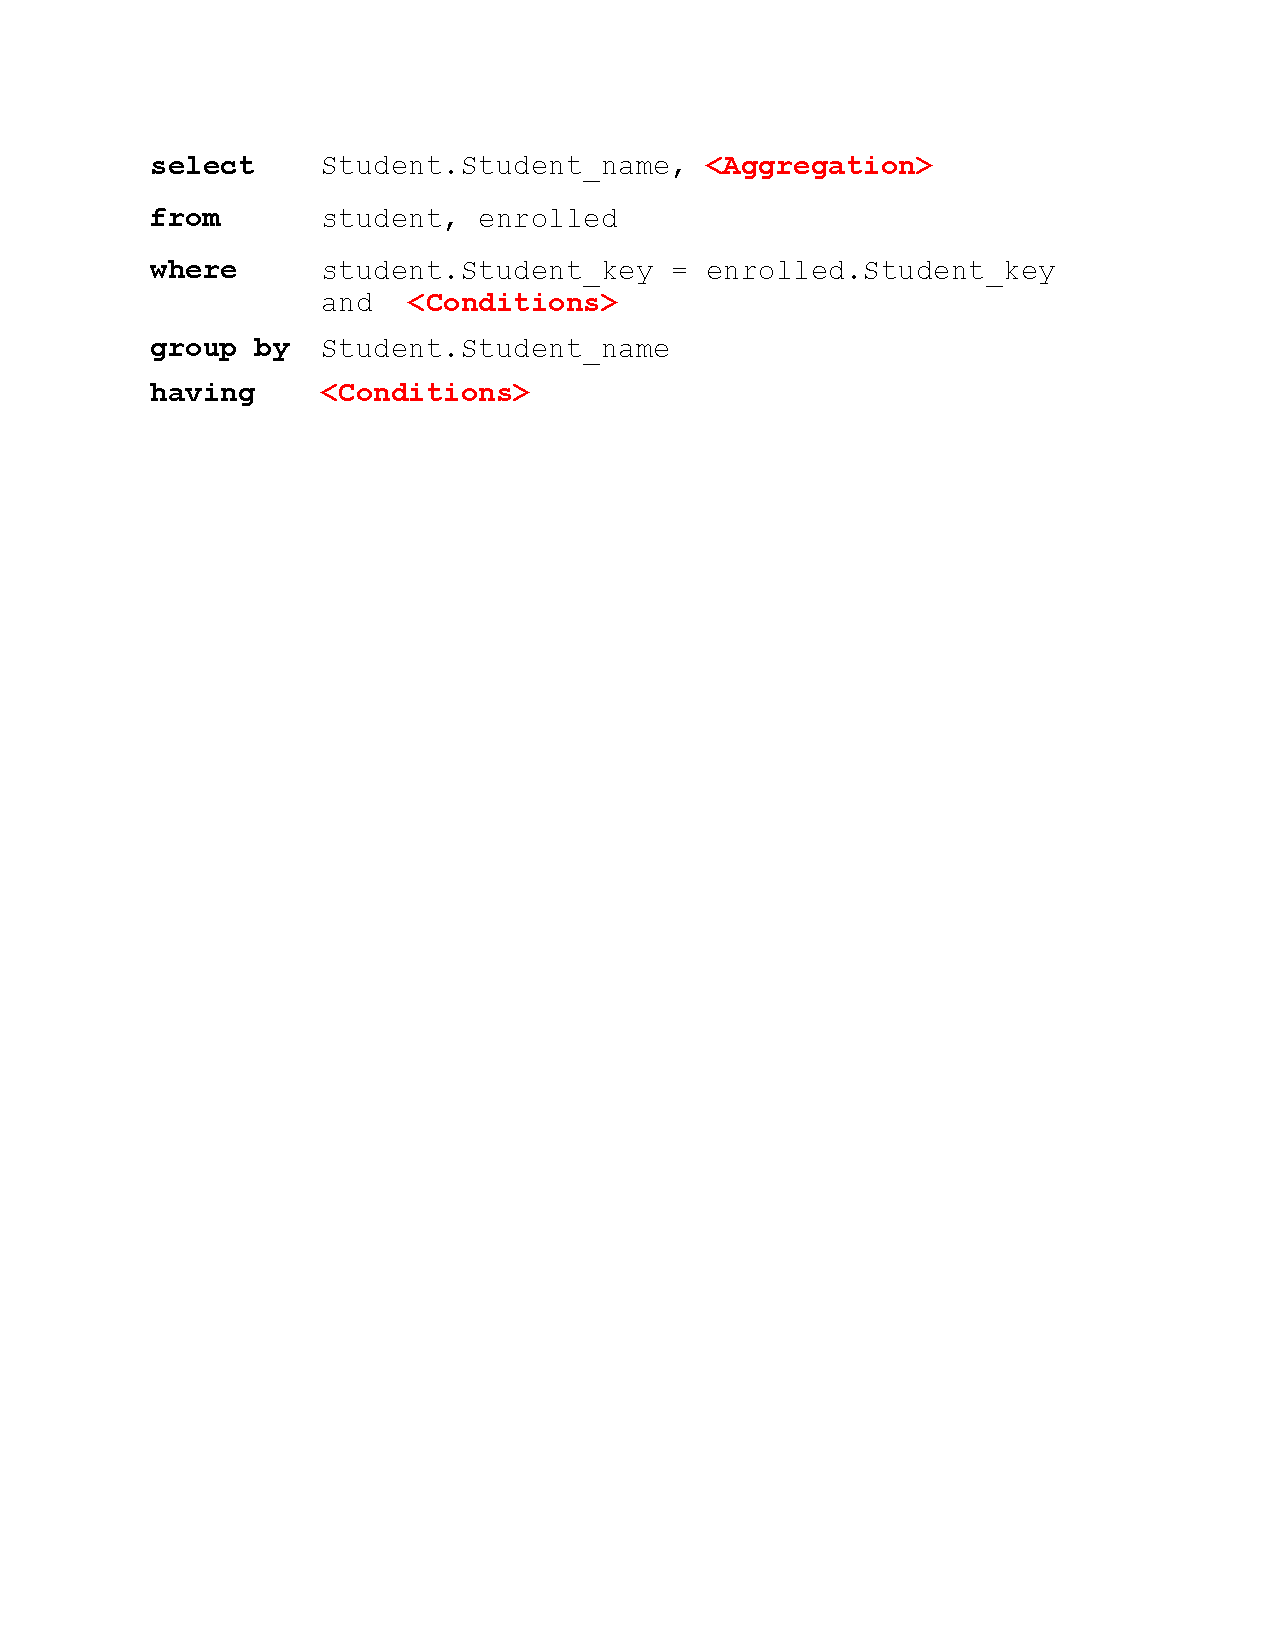
\includegraphics[width=0.45\textwidth]{sql_skeleton.pdf}
	\caption{The SQL skeleton created for the motivating example
in Figure~\ref{fig:motivating}.}
	\label{fig:skeleton}
\end{figure}

Figure~\ref{fig:skeleton} shows the created query skeleton
for the motivating example in Figure~\ref{fig:motivating}.
In this skeleton,  three unknown structures represented by
$<$Aggregation$>$ or $<$Conditions$>$ are in red, and
will be filled in the next phase. \todo{revise text}


\todo{how to create group by}

% which indicates aggregation and group by.

%After determining the table set and joining columns,
%the next step is to identify potential column names on which the result would be projected. If a
%column in the output table  does not appear in any input table's column list, this output column must
%be produced by aggregation. Our algorithm keeps track of these columns and appends a \CodeIn{group by} ... \CodeIn{having} ...
%clause to the query skeleton.

%\end{itemize}

%In summary, this step infers three parts as a query skeleton: tables used in constructing a SQL query, joining conditions
%to connect the input tables, and a list of columns to project the output results.

%It is worth noting that the results obtained from the above steps are not \textit{safe} in
%terms that they may miss some valid SQL queries. 

%We made the above assumption for the sake of tractability,
%since in theory, the bound of table number in a SQL query is $O(n_t!)$, where $n_t$ is the number of given tables;
%while the bound of possible number of join is $O(c_t^2)$ and the bound of the number of conditions is $O(n_t!n_tc_t^2)<O(n_t^3c_t^2)$.

%\subsubsection{Inferring Output Table Schema}

%Lacks schema


%while the bound of possible number of join is $O(c_t^2)$ and the bound of the number of conditions is $O(n_t!n_tc_t^2)<O(n_t^3c_t^2)$.


